General structure and tasks of an early detection system were already described in chapter \ref{early_detection_system}.
As it was mentioned before, an early detection system consists of two different components:

\begin{enumerate} 
    \item Several small embedded devices, deployed in the field. 
        They capture images with thermal camera, process them and send results over wireless network.
    \item One gateway, which is receiving results, and relays them to an application server over internet connection.
\end{enumerate} 

In this chapter we focus on the structure and design of deployed embedded system,both from hardware and firmware point of perspective.
We also describe construction of an application server, how received data is processed, stored and presented.

The general block diagram of an embedded system with a thermal camera is presented on the Figure \ref{system_diagram} 

\begin{figure}[ht]
        \centering
        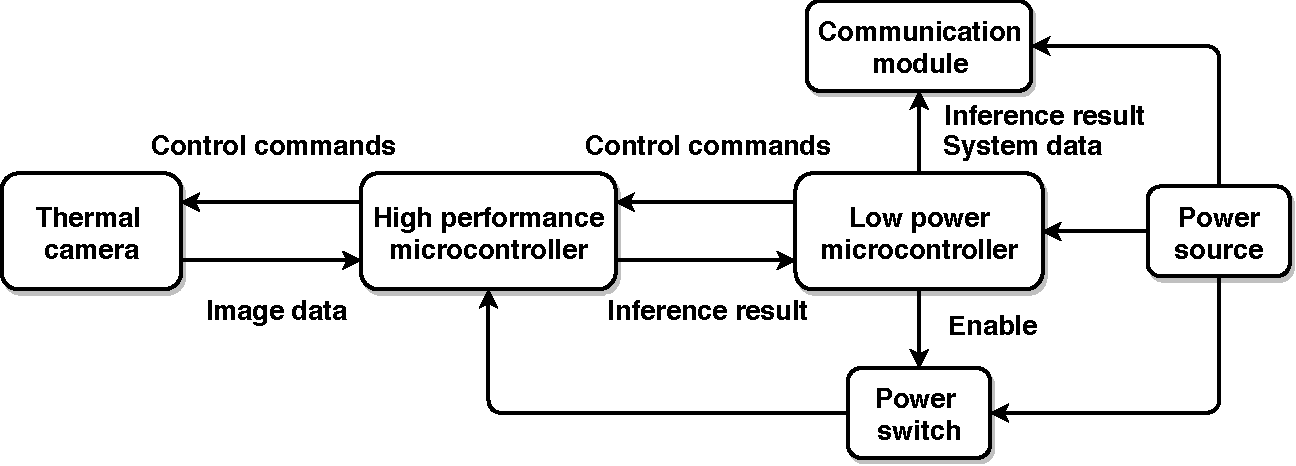
\includegraphics[width=1.0\linewidth]{system_diagram.pdf} 
        \caption{ General block diagram of an embedded system}
        \label{system_diagram}
\end{figure}

Embedded system will consist of two different microcontrollers with two distinct tasks, a thermal camera, PIR sensor, wireless communication module, power switch and battery.

Powerful, high performance microcontroller and thermal camera are turned off, to conserve battery life.
A less capable, but low power microcontroller will spend most the time in sleep, waiting for a trigger from PIR sensor.
PIR sensor will point in the same direction as the thermal camera and will detect any IR radiation of a passing object.

If an object passes PIR's field of vision, it triggers it, which in consequently wakes up a low power microcontroller.
Microcontroller will then enable power supply to high performance microcontroller and thermal camera, and send a command request for image capture and processing.

Thermal camera only communicates with high performance microcontroller, which configures it and requests image data.
That data is then inputted into neural network algorithm and an probability results are then returned to a low power microcontroller.
low power microcontroller then packs the data and sends it over radio through wireless communication module.
Power source to high performance microcontroller and thermal camera is then turned of to conserve power.
Diagram of described procedure can also be seen on Figure \ref{system_flow}.

\begin{figure}[ht]
        \centering
        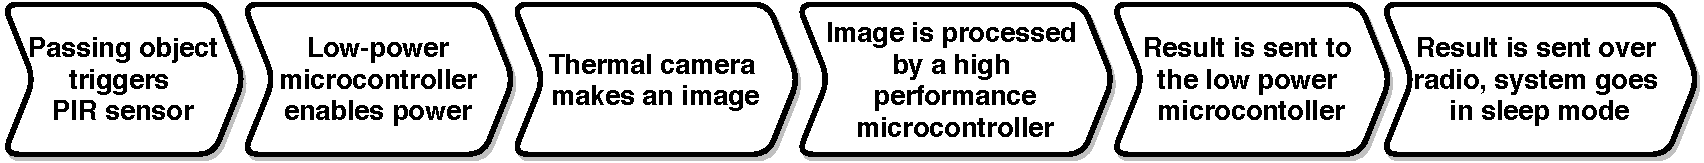
\includegraphics[width=1.0\linewidth]{system_flow.pdf} 
        \caption{ Diagram describing behavior of embedded early detection system} 
        \label{system_flow}
\end{figure}


\section{ Hardware}

In this section we present concrete components that we used to implement the embedded part of the early detection system.
Hardware version of embedded system diagram is presented on the Figure \ref{hardware_diagram}.
It should be noted that we did not include specific power source into the diagram.
Wisent Edge tracker board is general enough to work with different power sources, such as non-chargeable or chargeable batteries and or solar cells.

\begin{figure}[ht]
        \centering
        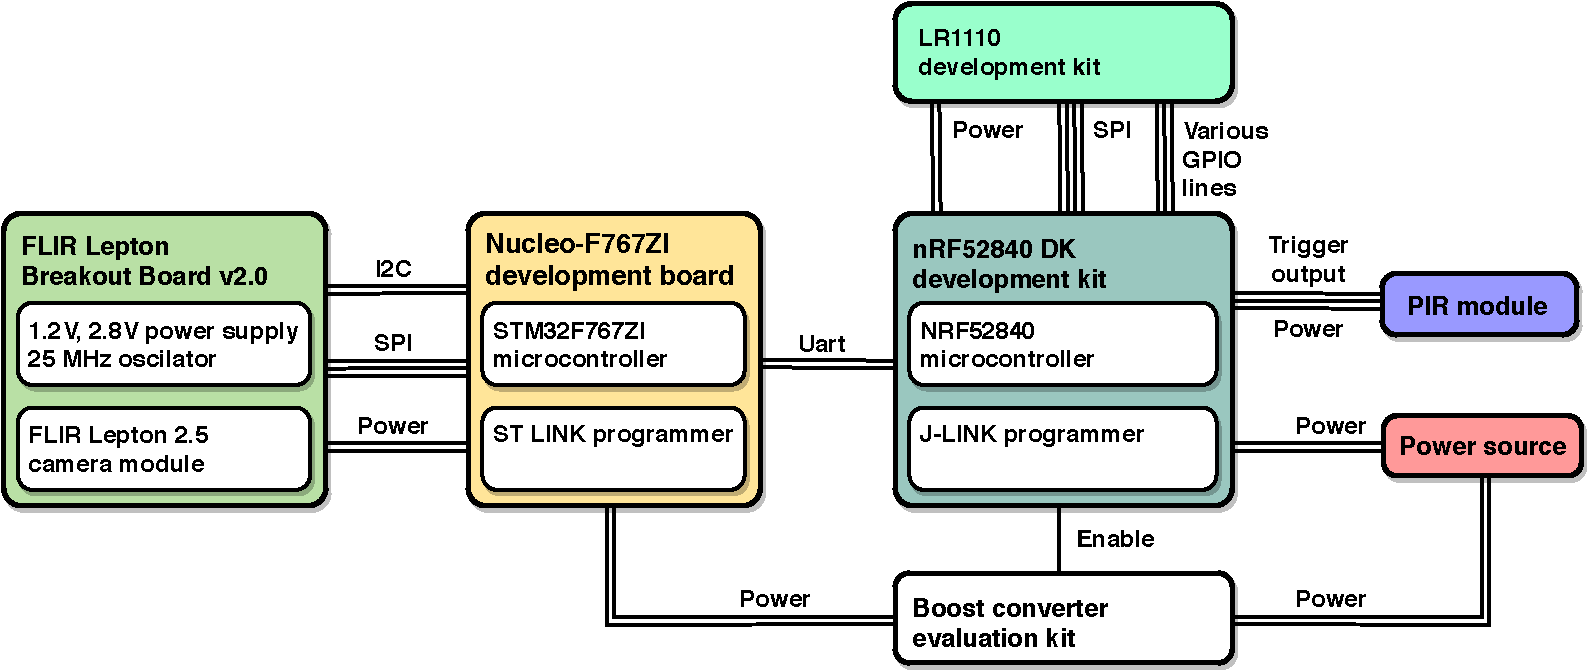
\includegraphics[width=1.0\linewidth]{hardware_diagram.pdf} 
        \caption{ Hardware diagram of embedded early detection system} 
        \label{hardware_diagram}
\end{figure}

\subsection{ Nucleo-F767ZI}

Nucleo-F767ZI (seen on Figure \ref{nucleo}) is a development board made by STMicroelectronics.
Board features STM32F767ZI microcontroller which has 2 \si{\mega\byte} of flash, 512 \si{\kilo\byte} of SRAM and can operate at clock speed of 216 \si{\mega\hertz}.
It also features different memory caches and flash accelerator, which provide extra boost in performance.
It is convenient to program it, as it includes on board ST-LINK programmer circuit.

We chose this microcontroller simply because it is one of more powerful general purpose microcontrollers on the market.
As we knew that neural networks are computationally expensive to compute and that models can be quite large in terms of memory, we selected it, knowing that we can always scale down if we have to.

\begin{figure}[ht]
        \centering
        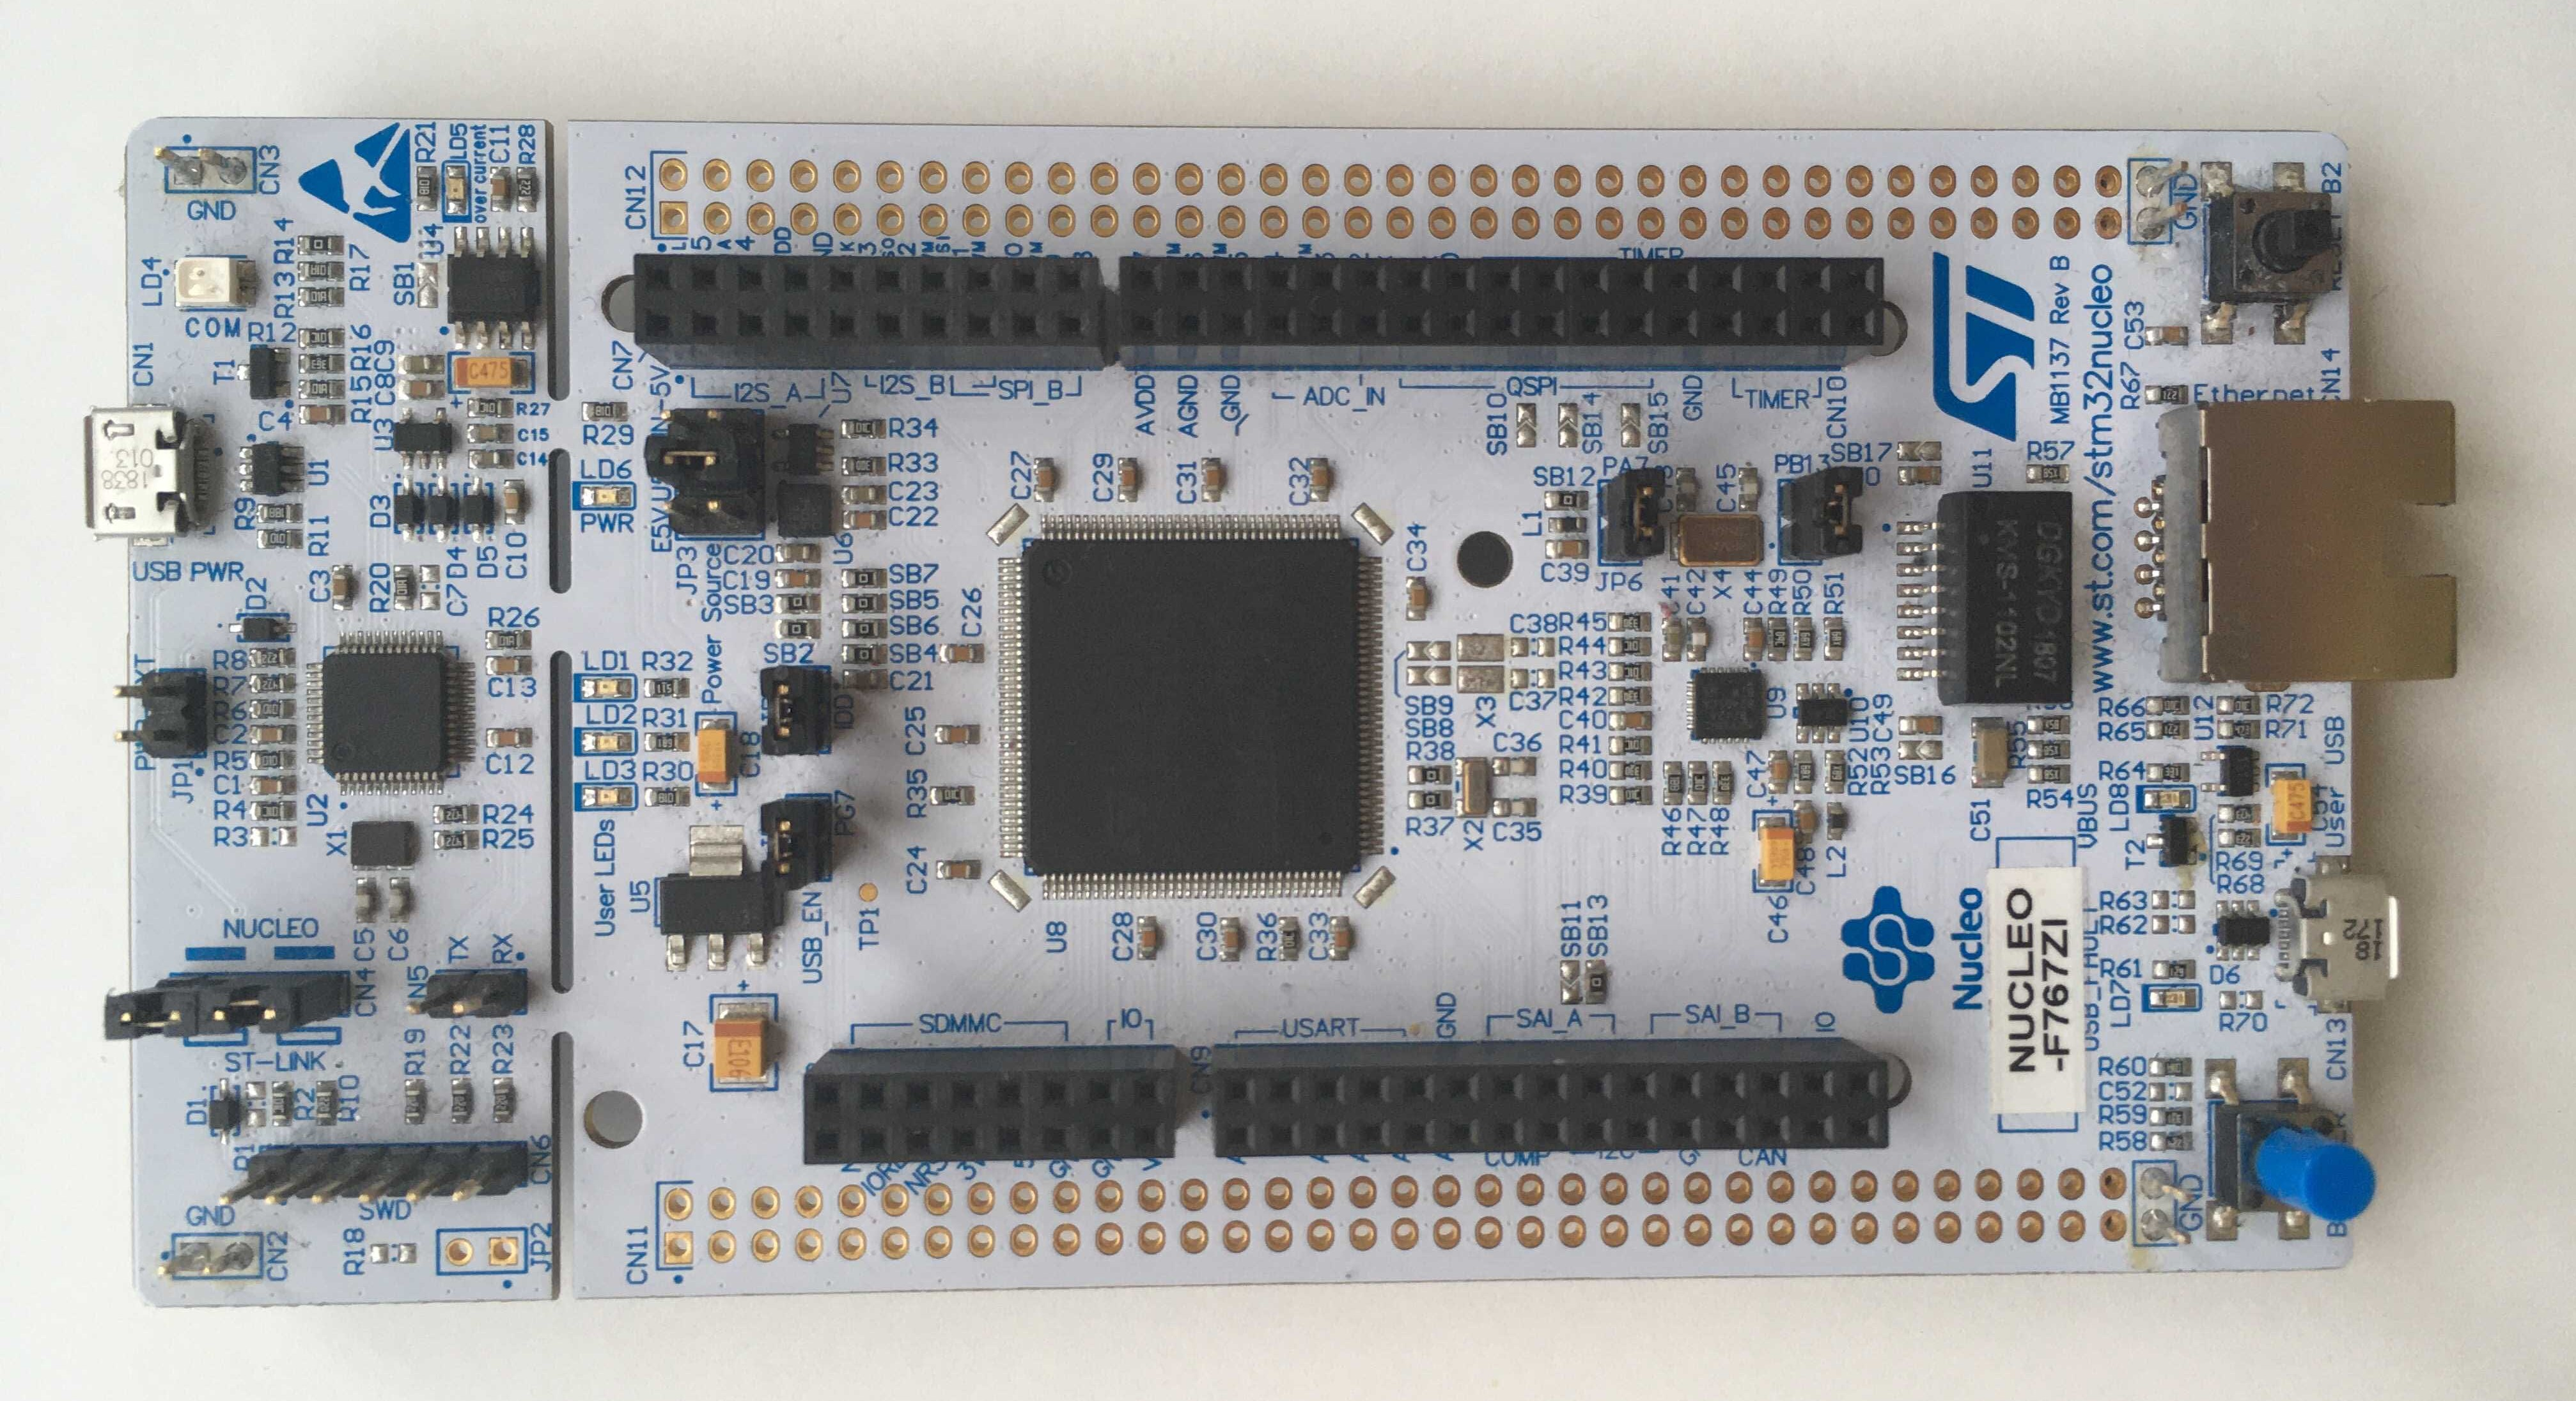
\includegraphics[width=1.0\linewidth]{nucleo.pdf} 
        \caption{ Nucleo-F767ZI development board} 
        \label{nucleo}
\end{figure}


\subsection{ Wisent Edge tracker}



    block diagram

\subsection{ Flir Lepton 2.5}
\subsection{ PIR Sensor}

%    4.1 Hardware 
%        block ampak tokrat s dejanskimi komponentami 
%        STM32F767
%        WISENT BOARD,IRNASOV PRODUKT PREDSTAVI , SMART PARKS OPEN COLLARJK
%
%        FLIR CAMERA 2.5, describe communication protocol.
%        TRIGGER COMPONENT? PIR
%
%        Choice of components, why we chose stmf7, description of components
%        Probably each component needs its section, 
%
%\chapter{Planning and design of early warning system}
%\section{ Hardware}
%\subsection{ Nucleo-F767zi}
%\subsection{ Wisent Edge tracker}
%    block diagram
%\subsection{ Flir Lepton 2.5}
%\subsection{ PIR Sensor}
%
%\section{ Firmware}
%\subsection{ Build system}
%\subsection{ Running inference on a microcontoller}
%\subsection{ Wisent board control firmware}
%
%\section{ Server side components/software}
%\subsection{ TTN}
%\subsection{ NODE-RED}
%\subsection{ InfluxDB}
%\subsection{ Grafana}
%
%
%
%
%
%
%
%
%
%
%
%
%Part of this thesis was concerned with porting TFLite Micro to \textbf{libopencm3}, our platform of choice.
%To compile source files and build binaries TFLite Micro uses build automation tool \textbf{GNU Make}.
%One large makefile that includes several platform specific makefiles dictates how firmware is built.
%By providing command line arguments users decide which example has to be compiled and for which platform.
%The build system makes some assumptions about locations of the platform specific files, which in case of example projects are scattered over GitHub repository.
%This and several other reasons make library hard to use when porting it to a new platform.
%In section TODO ADD REFERENCE we describe our build system that keeps library and application specific code separated in a clear and concise manner.
%
